% Options for packages loaded elsewhere
\PassOptionsToPackage{unicode}{hyperref}
\PassOptionsToPackage{hyphens}{url}
\PassOptionsToPackage{dvipsnames,svgnames,x11names}{xcolor}
%
\documentclass[
  a4paperpaper,
]{article}

\usepackage{amsmath,amssymb}
\usepackage{iftex}
\ifPDFTeX
  \usepackage[T1]{fontenc}
  \usepackage[utf8]{inputenc}
  \usepackage{textcomp} % provide euro and other symbols
\else % if luatex or xetex
  \usepackage{unicode-math}
  \defaultfontfeatures{Scale=MatchLowercase}
  \defaultfontfeatures[\rmfamily]{Ligatures=TeX,Scale=1}
\fi
\usepackage{lmodern}
\ifPDFTeX\else  
    % xetex/luatex font selection
\fi
% Use upquote if available, for straight quotes in verbatim environments
\IfFileExists{upquote.sty}{\usepackage{upquote}}{}
\IfFileExists{microtype.sty}{% use microtype if available
  \usepackage[]{microtype}
  \UseMicrotypeSet[protrusion]{basicmath} % disable protrusion for tt fonts
}{}
\makeatletter
\@ifundefined{KOMAClassName}{% if non-KOMA class
  \IfFileExists{parskip.sty}{%
    \usepackage{parskip}
  }{% else
    \setlength{\parindent}{0pt}
    \setlength{\parskip}{6pt plus 2pt minus 1pt}}
}{% if KOMA class
  \KOMAoptions{parskip=half}}
\makeatother
\usepackage{xcolor}
\usepackage[top=30mm,left=20mm,heightrounded]{geometry}
\setlength{\emergencystretch}{3em} % prevent overfull lines
\setcounter{secnumdepth}{-\maxdimen} % remove section numbering
% Make \paragraph and \subparagraph free-standing
\ifx\paragraph\undefined\else
  \let\oldparagraph\paragraph
  \renewcommand{\paragraph}[1]{\oldparagraph{#1}\mbox{}}
\fi
\ifx\subparagraph\undefined\else
  \let\oldsubparagraph\subparagraph
  \renewcommand{\subparagraph}[1]{\oldsubparagraph{#1}\mbox{}}
\fi

\usepackage{color}
\usepackage{fancyvrb}
\newcommand{\VerbBar}{|}
\newcommand{\VERB}{\Verb[commandchars=\\\{\}]}
\DefineVerbatimEnvironment{Highlighting}{Verbatim}{commandchars=\\\{\}}
% Add ',fontsize=\small' for more characters per line
\newenvironment{Shaded}{}{}
\newcommand{\AlertTok}[1]{\textcolor[rgb]{1.00,0.33,0.33}{\textbf{#1}}}
\newcommand{\AnnotationTok}[1]{\textcolor[rgb]{0.42,0.45,0.49}{#1}}
\newcommand{\AttributeTok}[1]{\textcolor[rgb]{0.84,0.23,0.29}{#1}}
\newcommand{\BaseNTok}[1]{\textcolor[rgb]{0.00,0.36,0.77}{#1}}
\newcommand{\BuiltInTok}[1]{\textcolor[rgb]{0.84,0.23,0.29}{#1}}
\newcommand{\CharTok}[1]{\textcolor[rgb]{0.01,0.18,0.38}{#1}}
\newcommand{\CommentTok}[1]{\textcolor[rgb]{0.42,0.45,0.49}{#1}}
\newcommand{\CommentVarTok}[1]{\textcolor[rgb]{0.42,0.45,0.49}{#1}}
\newcommand{\ConstantTok}[1]{\textcolor[rgb]{0.00,0.36,0.77}{#1}}
\newcommand{\ControlFlowTok}[1]{\textcolor[rgb]{0.84,0.23,0.29}{#1}}
\newcommand{\DataTypeTok}[1]{\textcolor[rgb]{0.84,0.23,0.29}{#1}}
\newcommand{\DecValTok}[1]{\textcolor[rgb]{0.00,0.36,0.77}{#1}}
\newcommand{\DocumentationTok}[1]{\textcolor[rgb]{0.42,0.45,0.49}{#1}}
\newcommand{\ErrorTok}[1]{\textcolor[rgb]{1.00,0.33,0.33}{\underline{#1}}}
\newcommand{\ExtensionTok}[1]{\textcolor[rgb]{0.84,0.23,0.29}{\textbf{#1}}}
\newcommand{\FloatTok}[1]{\textcolor[rgb]{0.00,0.36,0.77}{#1}}
\newcommand{\FunctionTok}[1]{\textcolor[rgb]{0.44,0.26,0.76}{#1}}
\newcommand{\ImportTok}[1]{\textcolor[rgb]{0.01,0.18,0.38}{#1}}
\newcommand{\InformationTok}[1]{\textcolor[rgb]{0.42,0.45,0.49}{#1}}
\newcommand{\KeywordTok}[1]{\textcolor[rgb]{0.84,0.23,0.29}{#1}}
\newcommand{\NormalTok}[1]{\textcolor[rgb]{0.14,0.16,0.18}{#1}}
\newcommand{\OperatorTok}[1]{\textcolor[rgb]{0.14,0.16,0.18}{#1}}
\newcommand{\OtherTok}[1]{\textcolor[rgb]{0.44,0.26,0.76}{#1}}
\newcommand{\PreprocessorTok}[1]{\textcolor[rgb]{0.84,0.23,0.29}{#1}}
\newcommand{\RegionMarkerTok}[1]{\textcolor[rgb]{0.42,0.45,0.49}{#1}}
\newcommand{\SpecialCharTok}[1]{\textcolor[rgb]{0.00,0.36,0.77}{#1}}
\newcommand{\SpecialStringTok}[1]{\textcolor[rgb]{0.01,0.18,0.38}{#1}}
\newcommand{\StringTok}[1]{\textcolor[rgb]{0.01,0.18,0.38}{#1}}
\newcommand{\VariableTok}[1]{\textcolor[rgb]{0.89,0.38,0.04}{#1}}
\newcommand{\VerbatimStringTok}[1]{\textcolor[rgb]{0.01,0.18,0.38}{#1}}
\newcommand{\WarningTok}[1]{\textcolor[rgb]{1.00,0.33,0.33}{#1}}

\providecommand{\tightlist}{%
  \setlength{\itemsep}{0pt}\setlength{\parskip}{0pt}}\usepackage{longtable,booktabs,array}
\usepackage{calc} % for calculating minipage widths
% Correct order of tables after \paragraph or \subparagraph
\usepackage{etoolbox}
\makeatletter
\patchcmd\longtable{\par}{\if@noskipsec\mbox{}\fi\par}{}{}
\makeatother
% Allow footnotes in longtable head/foot
\IfFileExists{footnotehyper.sty}{\usepackage{footnotehyper}}{\usepackage{footnote}}
\makesavenoteenv{longtable}
\usepackage{graphicx}
\makeatletter
\def\maxwidth{\ifdim\Gin@nat@width>\linewidth\linewidth\else\Gin@nat@width\fi}
\def\maxheight{\ifdim\Gin@nat@height>\textheight\textheight\else\Gin@nat@height\fi}
\makeatother
% Scale images if necessary, so that they will not overflow the page
% margins by default, and it is still possible to overwrite the defaults
% using explicit options in \includegraphics[width, height, ...]{}
\setkeys{Gin}{width=\maxwidth,height=\maxheight,keepaspectratio}
% Set default figure placement to htbp
\makeatletter
\def\fps@figure{htbp}
\makeatother

\makeatletter
\makeatother
\makeatletter
\makeatother
\makeatletter
\@ifpackageloaded{caption}{}{\usepackage{caption}}
\AtBeginDocument{%
\ifdefined\contentsname
  \renewcommand*\contentsname{Table of contents}
\else
  \newcommand\contentsname{Table of contents}
\fi
\ifdefined\listfigurename
  \renewcommand*\listfigurename{List of Figures}
\else
  \newcommand\listfigurename{List of Figures}
\fi
\ifdefined\listtablename
  \renewcommand*\listtablename{List of Tables}
\else
  \newcommand\listtablename{List of Tables}
\fi
\ifdefined\figurename
  \renewcommand*\figurename{Figure}
\else
  \newcommand\figurename{Figure}
\fi
\ifdefined\tablename
  \renewcommand*\tablename{Table}
\else
  \newcommand\tablename{Table}
\fi
}
\@ifpackageloaded{float}{}{\usepackage{float}}
\floatstyle{ruled}
\@ifundefined{c@chapter}{\newfloat{codelisting}{h}{lop}}{\newfloat{codelisting}{h}{lop}[chapter]}
\floatname{codelisting}{Listing}
\newcommand*\listoflistings{\listof{codelisting}{List of Listings}}
\makeatother
\makeatletter
\@ifpackageloaded{caption}{}{\usepackage{caption}}
\@ifpackageloaded{subcaption}{}{\usepackage{subcaption}}
\makeatother
\makeatletter
\@ifpackageloaded{tcolorbox}{}{\usepackage[skins,breakable]{tcolorbox}}
\makeatother
\makeatletter
\@ifundefined{shadecolor}{\definecolor{shadecolor}{rgb}{.97, .97, .97}}
\makeatother
\makeatletter
\makeatother
\makeatletter
\makeatother
\ifLuaTeX
  \usepackage{selnolig}  % disable illegal ligatures
\fi
\IfFileExists{bookmark.sty}{\usepackage{bookmark}}{\usepackage{hyperref}}
\IfFileExists{xurl.sty}{\usepackage{xurl}}{} % add URL line breaks if available
\urlstyle{same} % disable monospaced font for URLs
\hypersetup{
  pdftitle={Laser Exercise 3},
  colorlinks=true,
  linkcolor={blue},
  filecolor={Maroon},
  citecolor={Blue},
  urlcolor={Blue},
  pdfcreator={LaTeX via pandoc}}

\title{Laser Exercise 3}
\usepackage{etoolbox}
\makeatletter
\providecommand{\subtitle}[1]{% add subtitle to \maketitle
  \apptocmd{\@title}{\par {\large #1 \par}}{}{}
}
\makeatother
\subtitle{FYSS3552}
\author{}
\date{}

\begin{document}
\maketitle
\ifdefined\Shaded\renewenvironment{Shaded}{\begin{tcolorbox}[boxrule=0pt, breakable, borderline west={3pt}{0pt}{shadecolor}, frame hidden, interior hidden, enhanced, sharp corners]}{\end{tcolorbox}}\fi

Available at \url{https://andry3vi.github.io/FYSS3552}

\hypertarget{problem-1}{%
\section{Problem 1}\label{problem-1}}

\hypertarget{a}{%
\subsection{a}\label{a}}

Let's considering laser separation of two isotopes using a 2-step laser
ionization scheme. The isotope shifts are 3 GHz for the first excitation
and 5 GHz for the second excitation step, respectively. Assuming a FWMH
laser bandwidth of \(\Delta_{\text{laser},1}=2\) GHz for the first step,
\(\Delta_{\text{laser},2}=3\) GHz for the second step and ignoring the
natural linewidth as well as any saturation of the transitions or
contributions from Doppler broadening, one wants to compute the
selectivity, i.e.~the ratio of the ion signal of the two isotopes when
both lasers frequencies are set resonant to one isotope : \[
    S=\frac{I_{M1}(\nu_0^{M1})}{I_{M2}(\nu_0^{M1})}
\] with \(I_{M1}(\nu_0^{M1})\) being the intensity of the isotope \(1\)
at its atomic resonance \(\nu_0^{M1}\) and \(I_{M2}(\nu_0^{M1})\) being
the intensity of the isotope \(M2\) at the atomic resonance of the
isotope \(M1\). Assuming a Gaussian intensity distribution of the form,
\[
    I(\sigma,\nu)=\frac{1}{\sigma\sqrt{2\pi}}e^{-\frac{(\nu-\nu_0)^2}{2\sigma^2}}
\] The intensity distributions for isotopes \(M1\) and \(M2\) in the
first step are respectively, \[ 
I_{M1}(\sigma_1,\nu)=\frac{1}{\sigma_1\sqrt{2\pi}}e^{-\frac{(\nu-\nu_0^{M1})^2}{2\sigma_1^2}}
\] \[
I_{M2}(\sigma_1,\nu)=\frac{1}{\sigma_1\sqrt{2\pi}}e^{-\frac{(\nu-\nu_0^{M2})^2}{2\sigma_1^2}}
\] with
\(\sigma_1=\frac{\Delta_{\text{laser},1}}{2\sqrt{2\text{ln}2}}\),
\(\nu_0^{M1}=0\) and \(\nu_0^{M2}=3\) GHz so
\(\mid \nu_0^{M1}-\nu_0^{M2} \mid_1=3\) GHz.

The intensity distributions for isotopes \(M1\) and \(M2\) in the second
step are respectively, \[ 
I_{M1}(\sigma_2,\nu)=\frac{1}{\sigma_2\sqrt{2\pi}}e^{-\frac{(\nu-\nu_0^{M1})^2}{2\sigma_2^2}}
\] \[
I_{M2}(\sigma_2,\nu)=\frac{1}{\sigma_2\sqrt{2\pi}}e^{-\frac{(\nu-\nu_0^{M2})^2}{2\sigma_2^2}}
\] with
\(\sigma_2=\frac{\Delta_{\text{laser},2}}{2\sqrt{2\text{ln}2}}\),
\(\nu_0^{M1}=0\) and \(\nu_0^{M2}=5\) GHz so
\(\mid \nu_0^{M1}-\nu_0^{M2} \mid_2=5\) GHz.

One obtains the following plots :

\begin{Shaded}
\begin{Highlighting}[]
\ImportTok{import}\NormalTok{ matplotlib.pyplot }\ImportTok{as}\NormalTok{ plt}
\ImportTok{import}\NormalTok{ numpy }\ImportTok{as}\NormalTok{ np}
\ImportTok{import}\NormalTok{ matplotlib.gridspec }\ImportTok{as}\NormalTok{ gridspec}

\KeywordTok{def}\NormalTok{ gauss(x,cen,wid,amp):}
    \ControlFlowTok{return}\NormalTok{ np.exp(}\OperatorTok{{-}}\DecValTok{1}\OperatorTok{*}\NormalTok{(x}\OperatorTok{{-}}\NormalTok{cen)}\OperatorTok{**}\DecValTok{2}\OperatorTok{/}\NormalTok{(}\DecValTok{2}\OperatorTok{*}\NormalTok{wid}\OperatorTok{**}\DecValTok{2}\NormalTok{))}\OperatorTok{/}\NormalTok{(wid}\OperatorTok{*}\NormalTok{np.sqrt(}\DecValTok{2}\OperatorTok{*}\NormalTok{np.pi))}
\NormalTok{size }\OperatorTok{=} \DecValTok{18}
\NormalTok{plt.rcParams[}\StringTok{\textquotesingle{}font.size\textquotesingle{}}\NormalTok{]}\OperatorTok{=}\NormalTok{size}
\NormalTok{fig\_plot }\OperatorTok{=}\NormalTok{ plt.figure(figsize}\OperatorTok{=}\NormalTok{(}\DecValTok{20}\NormalTok{,}\DecValTok{9}\NormalTok{),dpi}\OperatorTok{=}\DecValTok{100}\NormalTok{)}
\NormalTok{gs }\OperatorTok{=}\NormalTok{ gridspec.GridSpec(}\DecValTok{1}\NormalTok{, }\DecValTok{2}\NormalTok{, fig\_plot)}
\NormalTok{axs\_1step }\OperatorTok{=}\NormalTok{ fig\_plot.add\_subplot(gs[}\DecValTok{0}\NormalTok{, }\DecValTok{0}\NormalTok{])}
\NormalTok{axs\_2step }\OperatorTok{=}\NormalTok{ fig\_plot.add\_subplot(gs[}\DecValTok{0}\NormalTok{, }\DecValTok{1}\NormalTok{])}

\NormalTok{xx }\OperatorTok{=}\NormalTok{ np.linspace(}\OperatorTok{{-}}\DecValTok{5}\NormalTok{,}\DecValTok{10}\NormalTok{,}\DecValTok{1000}\NormalTok{)}

\NormalTok{yy\_M1 }\OperatorTok{=}\NormalTok{ gauss(xx,}\DecValTok{0}\NormalTok{,}\DecValTok{2}\OperatorTok{/}\NormalTok{(}\DecValTok{2}\OperatorTok{*}\NormalTok{np.sqrt(}\DecValTok{2}\OperatorTok{*}\NormalTok{np.log(}\DecValTok{2}\NormalTok{))),}\DecValTok{1}\NormalTok{)}
\NormalTok{yy\_M2 }\OperatorTok{=}\NormalTok{ gauss(xx,}\DecValTok{3}\NormalTok{,}\DecValTok{2}\OperatorTok{/}\NormalTok{(}\DecValTok{2}\OperatorTok{*}\NormalTok{np.sqrt(}\DecValTok{2}\OperatorTok{*}\NormalTok{np.log(}\DecValTok{2}\NormalTok{))),}\DecValTok{1}\NormalTok{)}

\NormalTok{axs\_1step.plot(xx,yy\_M1,}\StringTok{"b{-}"}\NormalTok{,linewidth}\OperatorTok{=}\DecValTok{2}\NormalTok{)}
\NormalTok{axs\_1step.plot(xx,yy\_M2,}\StringTok{"r{-}"}\NormalTok{,linewidth}\OperatorTok{=}\DecValTok{2}\NormalTok{)}

\NormalTok{yy\_M1 }\OperatorTok{=}\NormalTok{ gauss(xx,}\DecValTok{0}\NormalTok{,}\DecValTok{3}\OperatorTok{/}\NormalTok{(}\DecValTok{2}\OperatorTok{*}\NormalTok{np.sqrt(}\DecValTok{2}\OperatorTok{*}\NormalTok{np.log(}\DecValTok{2}\NormalTok{))),}\DecValTok{1}\NormalTok{)}
\NormalTok{yy\_M2 }\OperatorTok{=}\NormalTok{ gauss(xx,}\DecValTok{5}\NormalTok{,}\DecValTok{3}\OperatorTok{/}\NormalTok{(}\DecValTok{2}\OperatorTok{*}\NormalTok{np.sqrt(}\DecValTok{2}\OperatorTok{*}\NormalTok{np.log(}\DecValTok{2}\NormalTok{))),}\DecValTok{1}\NormalTok{)}

\NormalTok{axs\_2step.plot(xx,yy\_M1,}\StringTok{"b{-}"}\NormalTok{,linewidth}\OperatorTok{=}\DecValTok{2}\NormalTok{)}
\NormalTok{axs\_2step.plot(xx,yy\_M2,}\StringTok{"r{-}"}\NormalTok{,linewidth}\OperatorTok{=}\DecValTok{2}\NormalTok{)}

\NormalTok{axs\_1step.set\_xlabel(}\VerbatimStringTok{r"Frequency w.r.t. $\textbackslash{}nu\_0\^{}}\SpecialCharTok{\{M1\}}\VerbatimStringTok{$ [GHz]"}\NormalTok{)}
\NormalTok{axs\_2step.set\_xlabel(}\VerbatimStringTok{r"Frequency w.r.t. $\textbackslash{}nu\_0\^{}}\SpecialCharTok{\{M1\}}\VerbatimStringTok{$ [GHz]"}\NormalTok{)}

\NormalTok{axs\_1step.set\_ylabel(}\VerbatimStringTok{r"Intensity [n.u.]"}\NormalTok{)}
\NormalTok{axs\_2step.set\_ylabel(}\VerbatimStringTok{r"Intensity [n.u.]"}\NormalTok{)}

\NormalTok{plt.show()}
\end{Highlighting}
\end{Shaded}

\begin{figure}[H]

{\centering 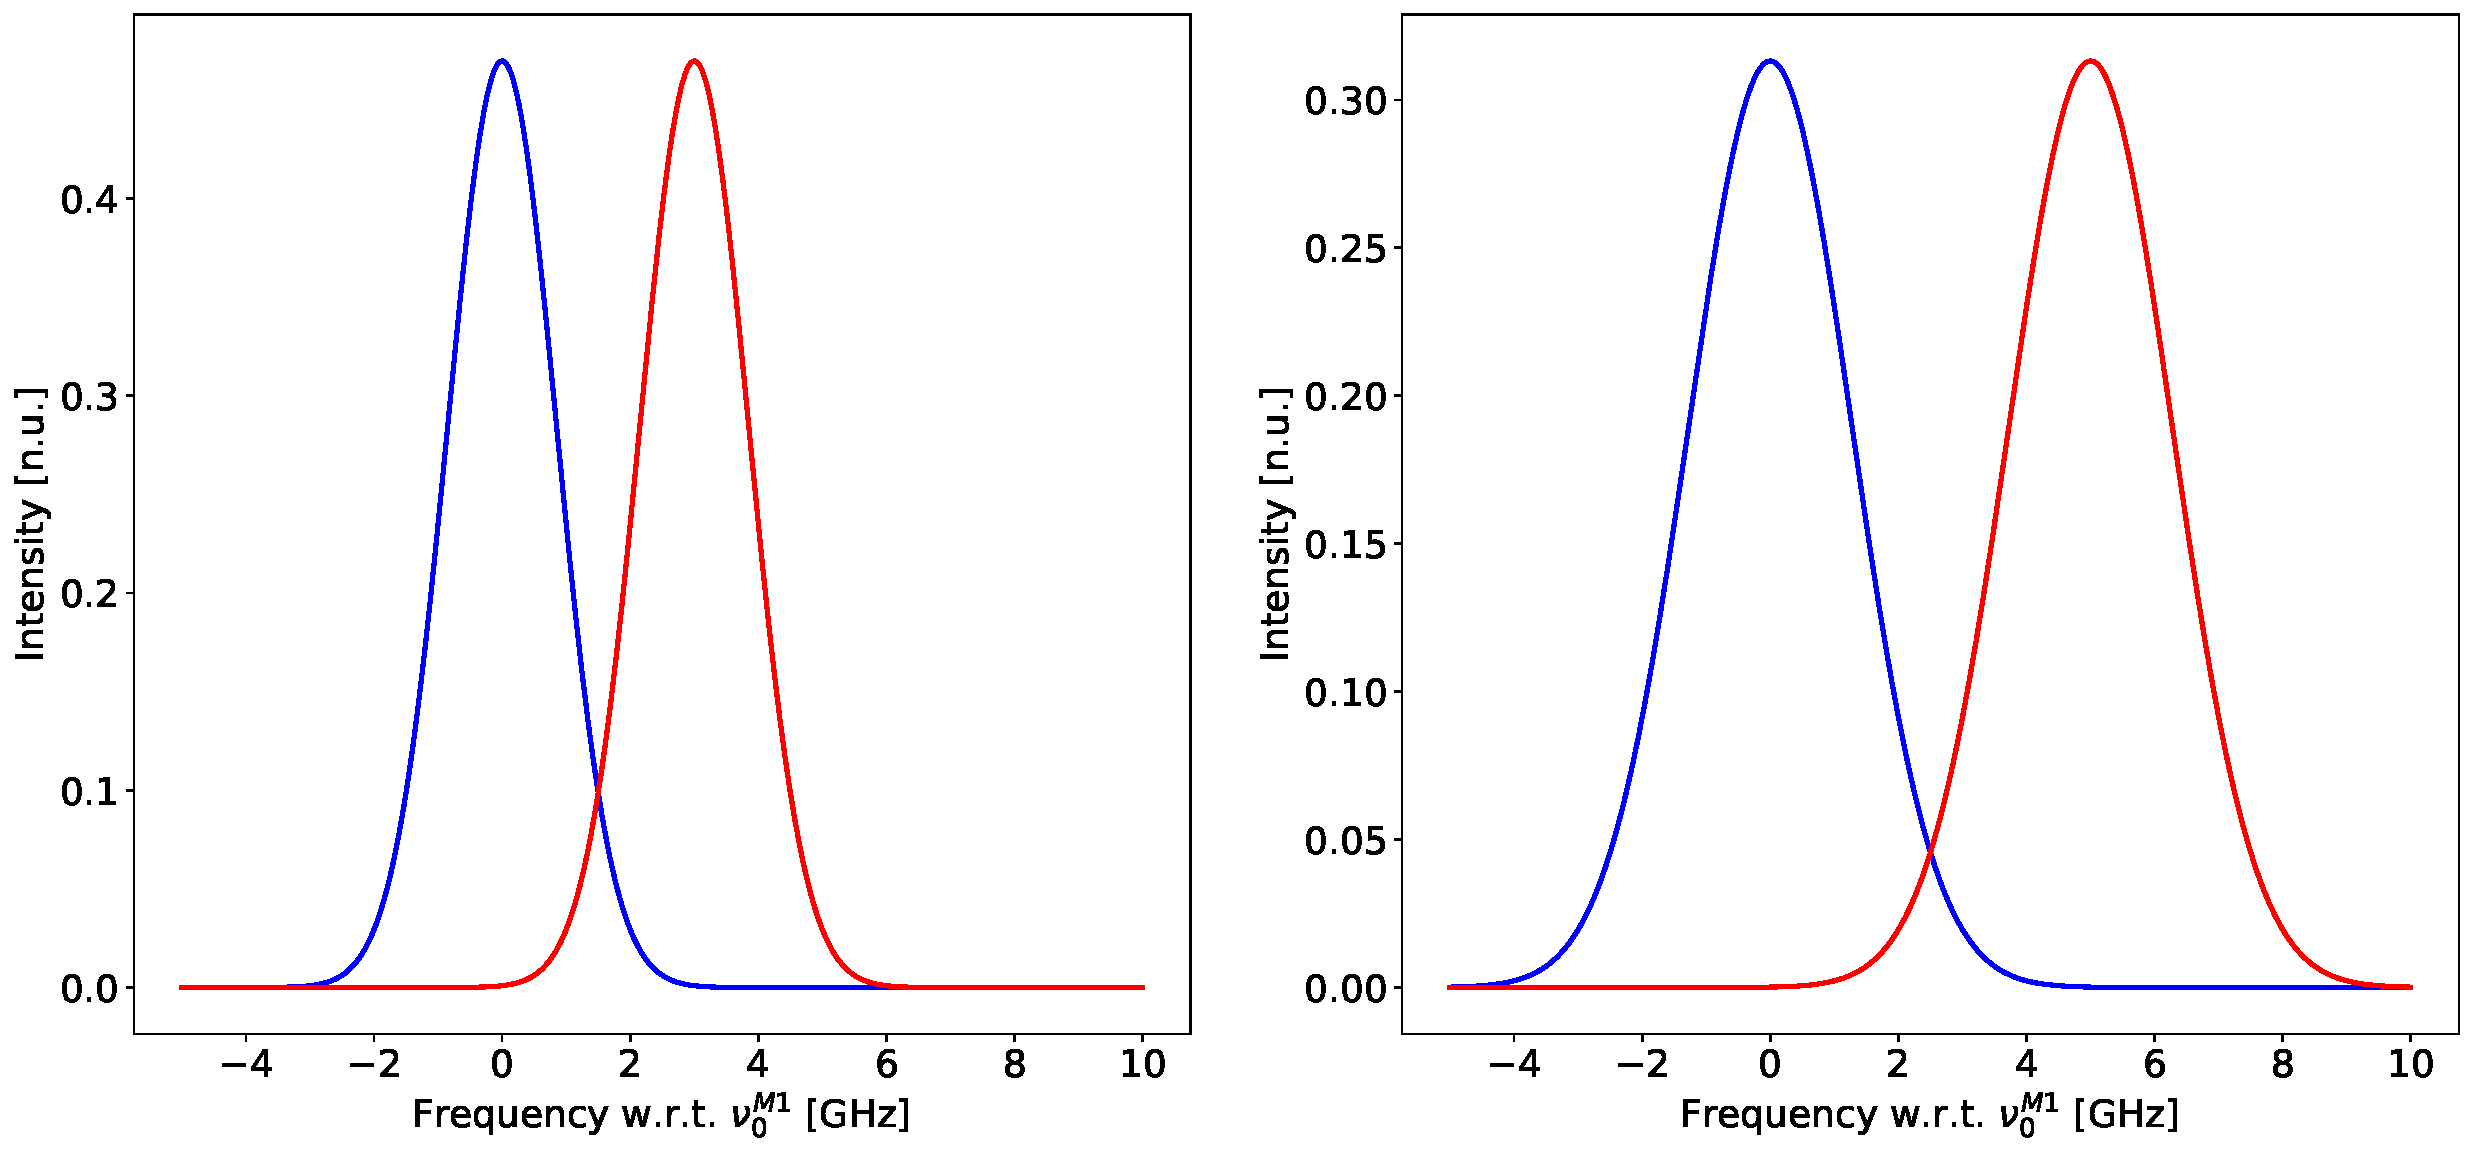
\includegraphics{Exercise3_files/figure-pdf/fig-iso-output-1.pdf}

}

\caption{\label{fig-iso}Isotope signals intensity distribution. In blue
figures the intensity distribution of the isotope of interest \(M1\) and
in red the intensity distribution of the other isotope \(M2\). The first
plot corresponds to the intensities for the first step \((left)\). The
second plot corresponds to the intensities for the second step
\((right)\)}

\end{figure}

The isotope signal ratios are then computed. The selectivity for the
first step is: \[
    S_1=e^{\frac{3\text{GHz}^2}{2\sigma_1^2}}=512
\] And the one for the second step is : \[
    S_2=e^{\frac{5\text{GHz}^2}{2\sigma_2^2}}=2212
\]

The total selectivity is in the end : \[
    S=S_1S_2
\] \[
\boxed{S=1132544}
\]

\hypertarget{problem-2}{%
\section{Problem 2}\label{problem-2}}

\hypertarget{a-1}{%
\subsection{a}\label{a-1}}

Assuming the resonance to be far from other contaminants the selectivity
is approximated: \[
    S\sim4\dfrac{\Delta^2}{\Gamma^2}
\] where \(\Delta\) correspond to the laser detuning between Kr isotopes
and \(\Gamma\) is extracted from the lifetime of the upper level: \[
    \Gamma=\dfrac{1}{2 \pi \tau}
\]

Hence \$S\sim\$1151.19 , using a three step resonance process the
overall selectivity would be \(S_{tot}=S^3\sim1.5\times10^9\), not
enough to resolve the natural abundance of \(^{81}\)Kr.

\hypertarget{b}{%
\subsection{b}\label{b}}

The photon momentum is computed as \[
    P_{ph.}=\dfrac{h}{\lambda}
\] and correspond to the the average momentum loss of the ion. Hence the
velocity is extracted as: \[
    v_{loss}=P_{ph.}/M_{^{81}\text{Kr}}=6.08\ \text{mm/s}
\]

\hypertarget{c}{%
\subsection{c}\label{c}}

Assuming resonance and high laser intensity the cycle time is: \[
T_{cycle} = 2\tau \left[ 1+\dfrac{I_{sat}}{I}\left( 1+4\dfrac{\Delta ^2}{\Gamma^2}\right)\right] \rightarrow 2\tau
\]

The maximum force on a particle is then given by:

\[
F=\dfrac{h}{2 \lambda \tau} = ma
\]

The acceleration can be then calculated: \[
a = -1.12 \times 10^5 \quad \text{m/s}
\]

\hypertarget{d}{%
\subsection{d}\label{d}}

Given the initial velocity of 300 m/s, the stopping time and distance
are given by the kinematic equation: \[
s = v_i t + \dfrac{at^2}{2}
\] hence \[
t = -\dfrac{v_i}{a} = 2.7 \text{ms}
\] and a distance of 0.4 m

\hypertarget{e}{%
\subsection{e}\label{e}}

The number of cycles is computed as : \[
    C = v/v_{loss}=49377
\]

Assuming a Doppler shift equal to \(\Gamma\) the velocity shift needed
is computed as: \[
    \delta v = \delta \nu_{D} \dfrac{c}{\nu_{0}} \sim 4.78\ \text{m/s}
\] Hence the number of cycle needed is \[
    C_{shift} = \dfrac{\delta v}{v_{loss}}\sim 786 
\]

\hypertarget{f}{%
\subsection{f}\label{f}}

The saturation intensities is computed as \[
    I_{s} = \dfrac{\pi h c }{3 \lambda^2 \tau} \times \dfrac{2F_{ex}+1}{ 3(2F_{gs}+1)} \sim 3.7\ \text{mW/cm}^2
\]

The trapping transition rate, is given by:

\[
T_{cycle} = \dfrac{1}{2\tau} \left[ 1+\dfrac{I_{sat}}{I}\left( 1+4\dfrac{\Delta ^2}{\Gamma^2}\right)\right]^{-1}
\]

Considering a used power of 20 mW/cm\(^2\) (retroreflected beam): \[
R=9.47 \text{MHz}
\]

\hypertarget{g}{%
\subsection{g}\label{g}}

Photon rate is given by scattering rate multiplied by detection
efficiencies: \[
N=R \varepsilon_{quantum}\varepsilon_{\Omega} = 23677
\]

Power is then given by: \[
P=\dfrac{h c}{\lambda} N = 5.8\times10^{-15}\quad\text{W}
\]



\end{document}
